% -*- coding: utf-8 -*-
\documentclass[12pt]{article}

\usepackage{listings}
\usepackage{ctex}
\usepackage{graphicx}
\usepackage[a4paper, body={18cm,22cm}]{geometry}
\usepackage{amsmath,amssymb,amstext,wasysym,enumerate,graphicx}
\usepackage{float,abstract,booktabs,indentfirst,amsmath}
\usepackage{array}
\usepackage{booktabs} %调整表格线与上下内容的间隔
\usepackage{multirow}
\usepackage{diagbox}
\usepackage{color}%字体颜色包
\usepackage[colorlinks,linkcolor=blue,urlcolor=black,anchorcolor=blue,citecolor=blue,]{hyperref}%超链接包
\renewcommand\arraystretch{1.4}
\usepackage{indentfirst}
\setlength{\parindent}{2em}

\geometry{left=2.8cm,right=2.2cm,top=2.5cm,bottom=2.5cm}
%\geometry{left=3.18cm,right=3.18cm,top=2.54cm,bottom=2.54cm}

\graphicspath{{figures/}}

\title{\heiti 作业四. PubTator基因突变实体识别和Shell编程}

\begin{document}

	\maketitle
	
	\vspace{5cm}
	
	\begin{table}[h]
		\centering
		\begin{Large}
			\begin{tabular}{p{3cm} p{7cm}<{\centering}}
				学  \qquad  校: &  华中农业大学     \\ \cline{2-2}
				学院班级:      & 信息学院生信1801班   \\ \cline{2-2}
				姓  \qquad  名: & 邓启东 \\ \cline{2-2}
				学  \qquad  号: & 2018317220103 \\ \cline{2-2}
				指导教师:       &夏静波 \\ \cline{2-2}
			\end{tabular}
		\end{Large}		
	\end{table}
	
	\newpage%一个新的页面

	\tableofcontents
	
	\newpage
	\section{实验目的}
通过shell编程得到检索词汇相关pmid,并且由id自动检索下载PubTator标注后的文献或摘要。并且识别其中的基因突变实体。然后我们选择其中我们认为比较重要的Chemical,Gene,Species三种实体两两之间的互作关系以Cytoscape可以识别的sif格式进行存储,并且利用Cytoscape进行可视化和相关分析。
	\section{实验材料与方法}
	\subsection{实验材料}
	\subsubsection{pubtator}
pubtator是一个基于web的工具,通过使用先进的文本挖掘技术来加速手动文献整理(例如注释生物实体及其关系)。作为一个一体化的系统,PubTator提供了对PubMed引文的一站式注释服务。
	\subsubsection{Entrez Direct}
	NCBI提供的Entrez Direct有着自己独特的检索语法和查询理念,和sql相似但语法上差距很大。\par
	esearch命令从NCBI检索符合条件的记录,并将结果的summary返回client的屏幕上,并没有下载结果。\par
	efetch的参数包括-db(指定数据库)和-query(查询条件)。条件用" "标记,包括带查询的关键字和字段名两部分,如"Solenysa[ScientificName]"表示学名为Solenysa的taxa或"933038[TaxId]"TaxId为933038的taxa。查询条件可用AND,OR等逻辑运算符组合。关键字也可使用*通配符。efetch命令则执行结果的下载,参数包括-format指定结果格式,如xml等。通常的检索过程是先esearch在执行efetch,两条命令用|连接,语句如跨行使用\\标记。
	本次试验主要采用的是esearch命令得到关键词的pmid。
	\subsubsection{curl}
	在Linux中curl是一个利用URL规则在命令行下工作的文件传输工具,可以说是一款很强大的http命令行工具。它支持文件的上传和下载,是综合传输工具,但按传统,习惯称url为下载工具。\par
	curl 是利用URL语法在命令行下工作的文件传输工具,1997年首次发行,支持文件上传和下载,结合shell脚本体验更棒。但按照传统习惯称 curl 为下载工具。\par
    curl 支持的通信协议有 有FTP、FTPS、HTTP、HTTPS、TFTP、SFTP 等等,支持的平台有 Linux、MacOSX、Darwin、Windows、DOS、FreeBSD等等。\par

	\subsubsection{cytoscape软件}
Cytoscape 是一个专注于开源网络可视化和分析的软件。它的核心是提供基础的功能布局和查询网络,并依据基本的数据的结合成可视化网络。\par
Cytoscape 源自系统生物学,用于将生物分子交互网络与高通量基因表达数据和其他的分子状态信息整合在一起,其最强大的功能还是用于大规模蛋白质-蛋白质相互作用、蛋白质-DNA和遗传交互作用的分析。\par
通过Cytoscape,可以在可视化的环境下将这些生物网络跟基因表达、基因型等各种分子状态信息整合在一起,还能将这些网络跟功能注释数据库链接在一起。\par
Cytoscape 的核心是网络,简单的网络图包括节点(node)和边(edge),每个节点可以是基因、miNRA或蛋白质等等;节点与节点之间的连接 (edge) 代表着这些节点之间的相互作用,包括蛋白与蛋白相互作用(pp),DNA与蛋白相互作用(pd)等。
	\subsection{实验方法}
	\subsubsection{查找关键词rice相关的pmid}
	使用:sudo apt install ncbi-entrez-direct安装esearch\par
	使用edirect找到感兴趣的关键词的pmidesearch -db pubmed -query "rice" | efetch -format uid >pmid\_MM.txt\par
	通过检索rice关键字,我们一共在Pubmeds上找到了94,942篇文献的id,存放于pmid\_MM.txt文件当中。
	\subsubsection{curl API接口爬取pubtator}
	使用shell编程中的curl逐篇爬取pubtator结果并且合并到文件result.txt中(代码见图\ref{mmmm})\par
\begin{figure}[H]
  \raggedleft
  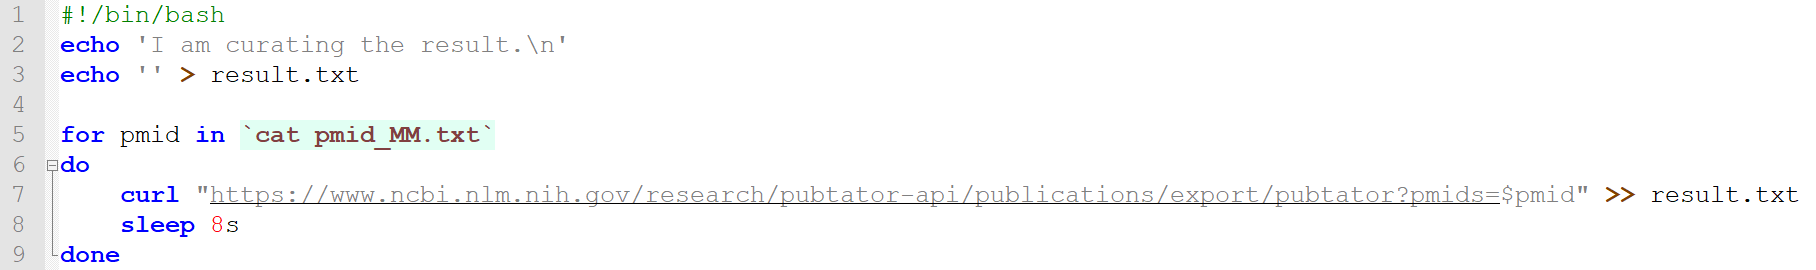
\includegraphics[scale=0.35]{./picture/curl.png} %1.png是图片文件的相对路径
  \caption{shell爬虫代码} %caption是图片的标题
  \label{mmmm} %此处的label相当于一个图片的专属标志,目的是方便上下文的引用
\end{figure}
	不足的是,这个爬虫由于需要设定休眠时间,且休眠时间最少也要1s才比较安全以免被认定为网络攻击。因此想要爬取94,942篇文献也许要整整两天的时间。可以使用multiprocessing包进行多线程管理,可以适当减少下载时间。
	在通过./NCBI3.sh运行该命令的时候,可能会出现以下问题(见图\ref{xxx})\par
	\begin{figure}[H]
  \centering
  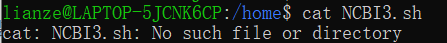
\includegraphics[scale=1.0]{./picture/question1.png} %1.png是图片文件的相对路径
  \caption{报错} %caption是图片的标题
  \label{xxx} %此处的label相当于一个图片的专属标志,目的是方便上下文的引用
\end{figure}	

原因可能是.sh从windows平台迁移到Linux平台出现的格式兼容问题,往往是文件格式是dos格式的缘故,改成unix 格式即可。用vim打开该sh文件,输入::set ff $\rightarrow$回车,显示fileformat=dos, $\rightarrow$重新设置下文件格式::set ff=unix $\rightarrow$ 保存退出: :wq,问题解决。\par
如果还有问题,有可能是虚拟机的bash目录为/bin/bash, 而不是默认的/usr/bin/bash。将脚本的内容第一行的命令解释器声明由\#!/usr/bin/bash改为\#!/bin/bash即可。\par
\subsubsection{文献处理}


我们由此得到了以下API格式的pubtator文献(图\ref{sss}):
\begin{figure}[H]
  \centering
  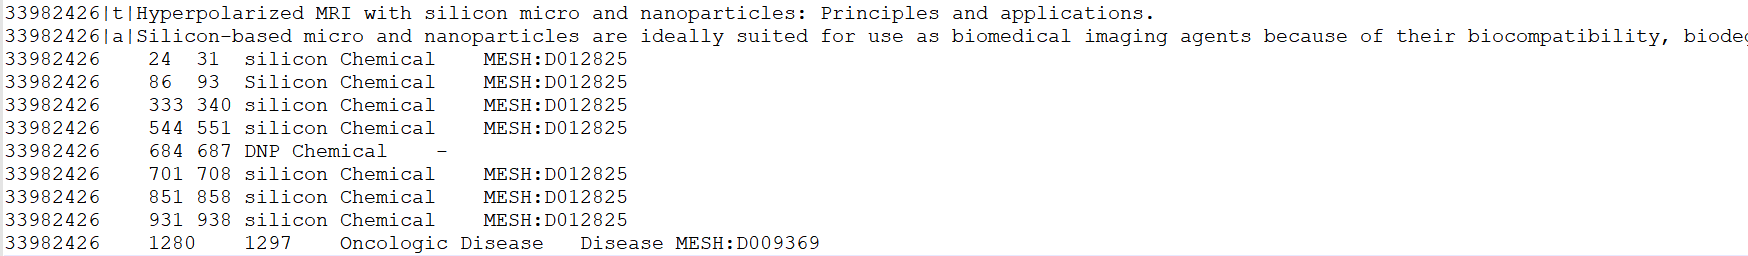
\includegraphics[scale=0.40]{./picture/example.png} %1.png是图片文件的相对路径
  \caption{数据格式} %caption是图片的标题
  \label{sss} %此处的label相当于一个图片的专属标志,目的是方便上下文的引用
\end{figure}	

对于每一篇文献,首行为标题行,第二行是摘要,之后的可以分成6列的是pubtator的标注。我们通过curl方式下载了一下午(约7小时),下载了5,395篇文献。
\subsection{pubmed.minR}
很高兴我们在网上发现了一个从 Pubmed Abstarct 文件挖掘文本/数据的包叫做pubmed.mineR\cite{2015pubmed},并且应该是可以提供pmid就能调用函数下载Abstract文件,也可以非常方便的将整个文本拆分成单词,除去空格、标点符号、常用单词,之后统计词频,绘制词云;也可以统计"基因频" ;还能够以“关键词” 和 “年份” 两个参数,得到 PubMed 中相关文章的数量,并可视化。
不过可惜的是,我们虽然成功的从pubmed上下载了10,000 文献摘要,并且成功用readabs函数读取,但是在后续统计词频和基因频的时候出现了报错。
\begin{figure}[H]
  \centering
  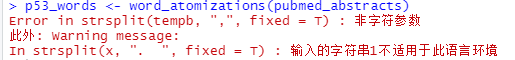
\includegraphics[scale=0.9]{./picture/error.png} %1.png是图片文件的相对路径
  \caption{报错} %caption是图片的标题
  \label{ssdd} %此处的label相当于一个图片的专属标志,目的是方便上下文的引用
\end{figure}	
后来发现是因为Pubmed发生了较大的改版而改pubmed.minR包没有更新导致。因此我们能利用这个比较方便的工具,转而需要自行撰写代码进行简单的分析。
\subsection{共句分析}
标题行大部分都是一个句号,极少数有多个句号,例如“Cellulomonas citrea sp. nov., isolated from paddy soil.”是一些学名或者缩写,本质上还是一个句子。因此一个标题我们就当作一句来看。\par
然后由于offset值是标题和摘要一起计算的,我们还要用变量title\_len记录下每个标题的长度。之后摘要标点的offset值要在其基础上加上标题长度。撰写函数,三次调用。最后把所有的断句标点(包括'.','?','!')的位置得到。\par
下面我们以第一篇摘要作为例子(还是图\ref{sss})。标题算上句点全长为85,由于观察发现标题是index从0开始,因此标题的最后一个句号的offset就是其index,为84。但是正文摘要部分第一个词Silicon的S位置可以从下方的Pubtator标注看出为86,也就是从1开始直接加上了前面标题的全长。也就是offset=正文第几个+标题全长。
撰写的代码可以给出剩下的6个分句标点的所有位置,并且一起储存于列表中(见图\ref{hhhh})。经过人工验证是正确的。
\begin{figure}[H]
  \centering
  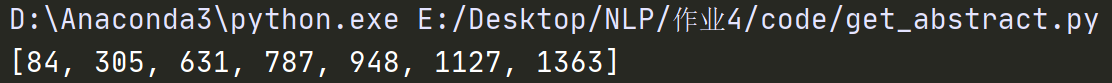
\includegraphics[scale=0.5]{./picture/list.png} %1.png是图片文件的相对路径
  \caption{第一篇的句点位置} %caption是图片的标题
  \label{hhhh} %此处的label相当于一个图片的专属标志,目的是方便上下文的引用
\end{figure}	
我们得到了分句子的标点offset位置信息,下面判断共句就比较简单了。因为pubtator已经给出了一些实体单词的开始位置和结束位置。只要保证两个词语被相同的一对标点框起来,便能反映两个词语共句。\par
我们成功撰写出了这个代码。代码的思路也非常简单,通过空行来区分每一篇文献,初始化一些参数,比如存放offset的一些集合或者列表,然后我们会读取到标题、正文。在这个过程中得到分句子标点的Offset信息。之后我们就读到了Pubtator的标注,我们会比较上下两行的内容是否在同一句,如果在的话我们就认为两者之间有相互作用。并且以Cytoscape软件可以读取的方式,即sif文件的格式整理起来(见下图\ref{ssaaass})。也就是三元组,左右是节点中间是相互作用名称。\par
\begin{figure}[H]
  \centering
  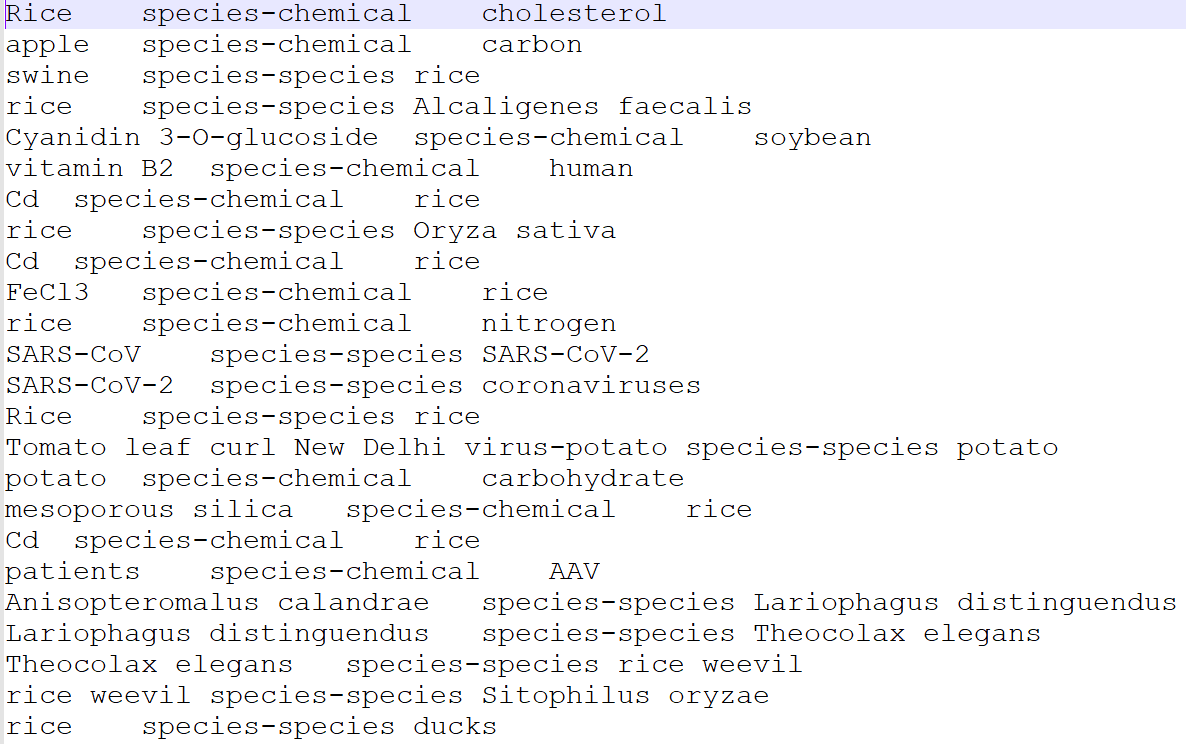
\includegraphics[scale=0.4]{./picture/form.png} %1.png是图片文件的相对路径
  \caption{sif格式(以tab分隔)} %caption是图片的标题
  \label{ssaaass} %此处的label相当于一个图片的专属标志,目的是方便上下文的引用
\end{figure}
但是这么多的实体两两组合,节点和边都十分的多,导致整个网络不是很清晰。因此我们分别关注三个实体:“Species”、“Gene”以及“Chemical”。\par
\subsubsection{Species的相互作用网络局部图}
首先关注物种,也就是我们只关注type为Species-Species、Species-Gene、Species-Chemical这三种相互作用。如上图\ref{ssaaass}的第二列所示,只有species-species、species-chemical、species-gene三种关系。然后我们把sif文件载入Cytoscape软件,并且设置每一个节点的半径和其度呈正比。并且将\textcolor{red}{species-chemical}设置为红色、\textcolor{green}{species-gene}设置为绿色、\textcolor{blue}{species-species}设置为蓝色。\par

\begin{figure}[H]
  \centering
  \includegraphics[scale=0.14]{./picture/Species.png} %1.png是图片文件的相对路径
  \caption{Species的相互作用网络图} %caption是图片的标题
  \label{xxxxxxx} %此处的label相当于一个图片的专属标志,目的是方便上下文的引用
\end{figure}
我们可以很明显的看到,中心的rice半径是最大的,也是一个hub节点,承载了非常大的流量,是整张图的中心。说明这也是被挖掘出来最多的物种,显然符合我们以rice为关键词检索到的文献的绘图预期。而且明显感受到\textcolor{blue}{物种-物种}之间关联出现居多,\textcolor{red}{物种-化学物质}也挺多,而\textcolor{green}{物种-基因}出现较少,原因从文本中可以看出,是基因本身就比较少,能够和物种共句子就更难了。\par
\subsubsection{Gene的相互作用网络局部图}
基因的相互作用网络局部图见图\ref{mmmss}。可以看到整个网络的规模和之前物种图相比小了很多。不仅如此,出现了以物种作为中心的独立网络图。这个局部位置主要有四个物种,rice、human、patients和Arabidopsis。其中:\textcolor{red}{基因-化学物质},\textcolor{blue}{基因-基因},\textcolor{green}{基因-物种}。
\begin{figure}[H]
  \centering
  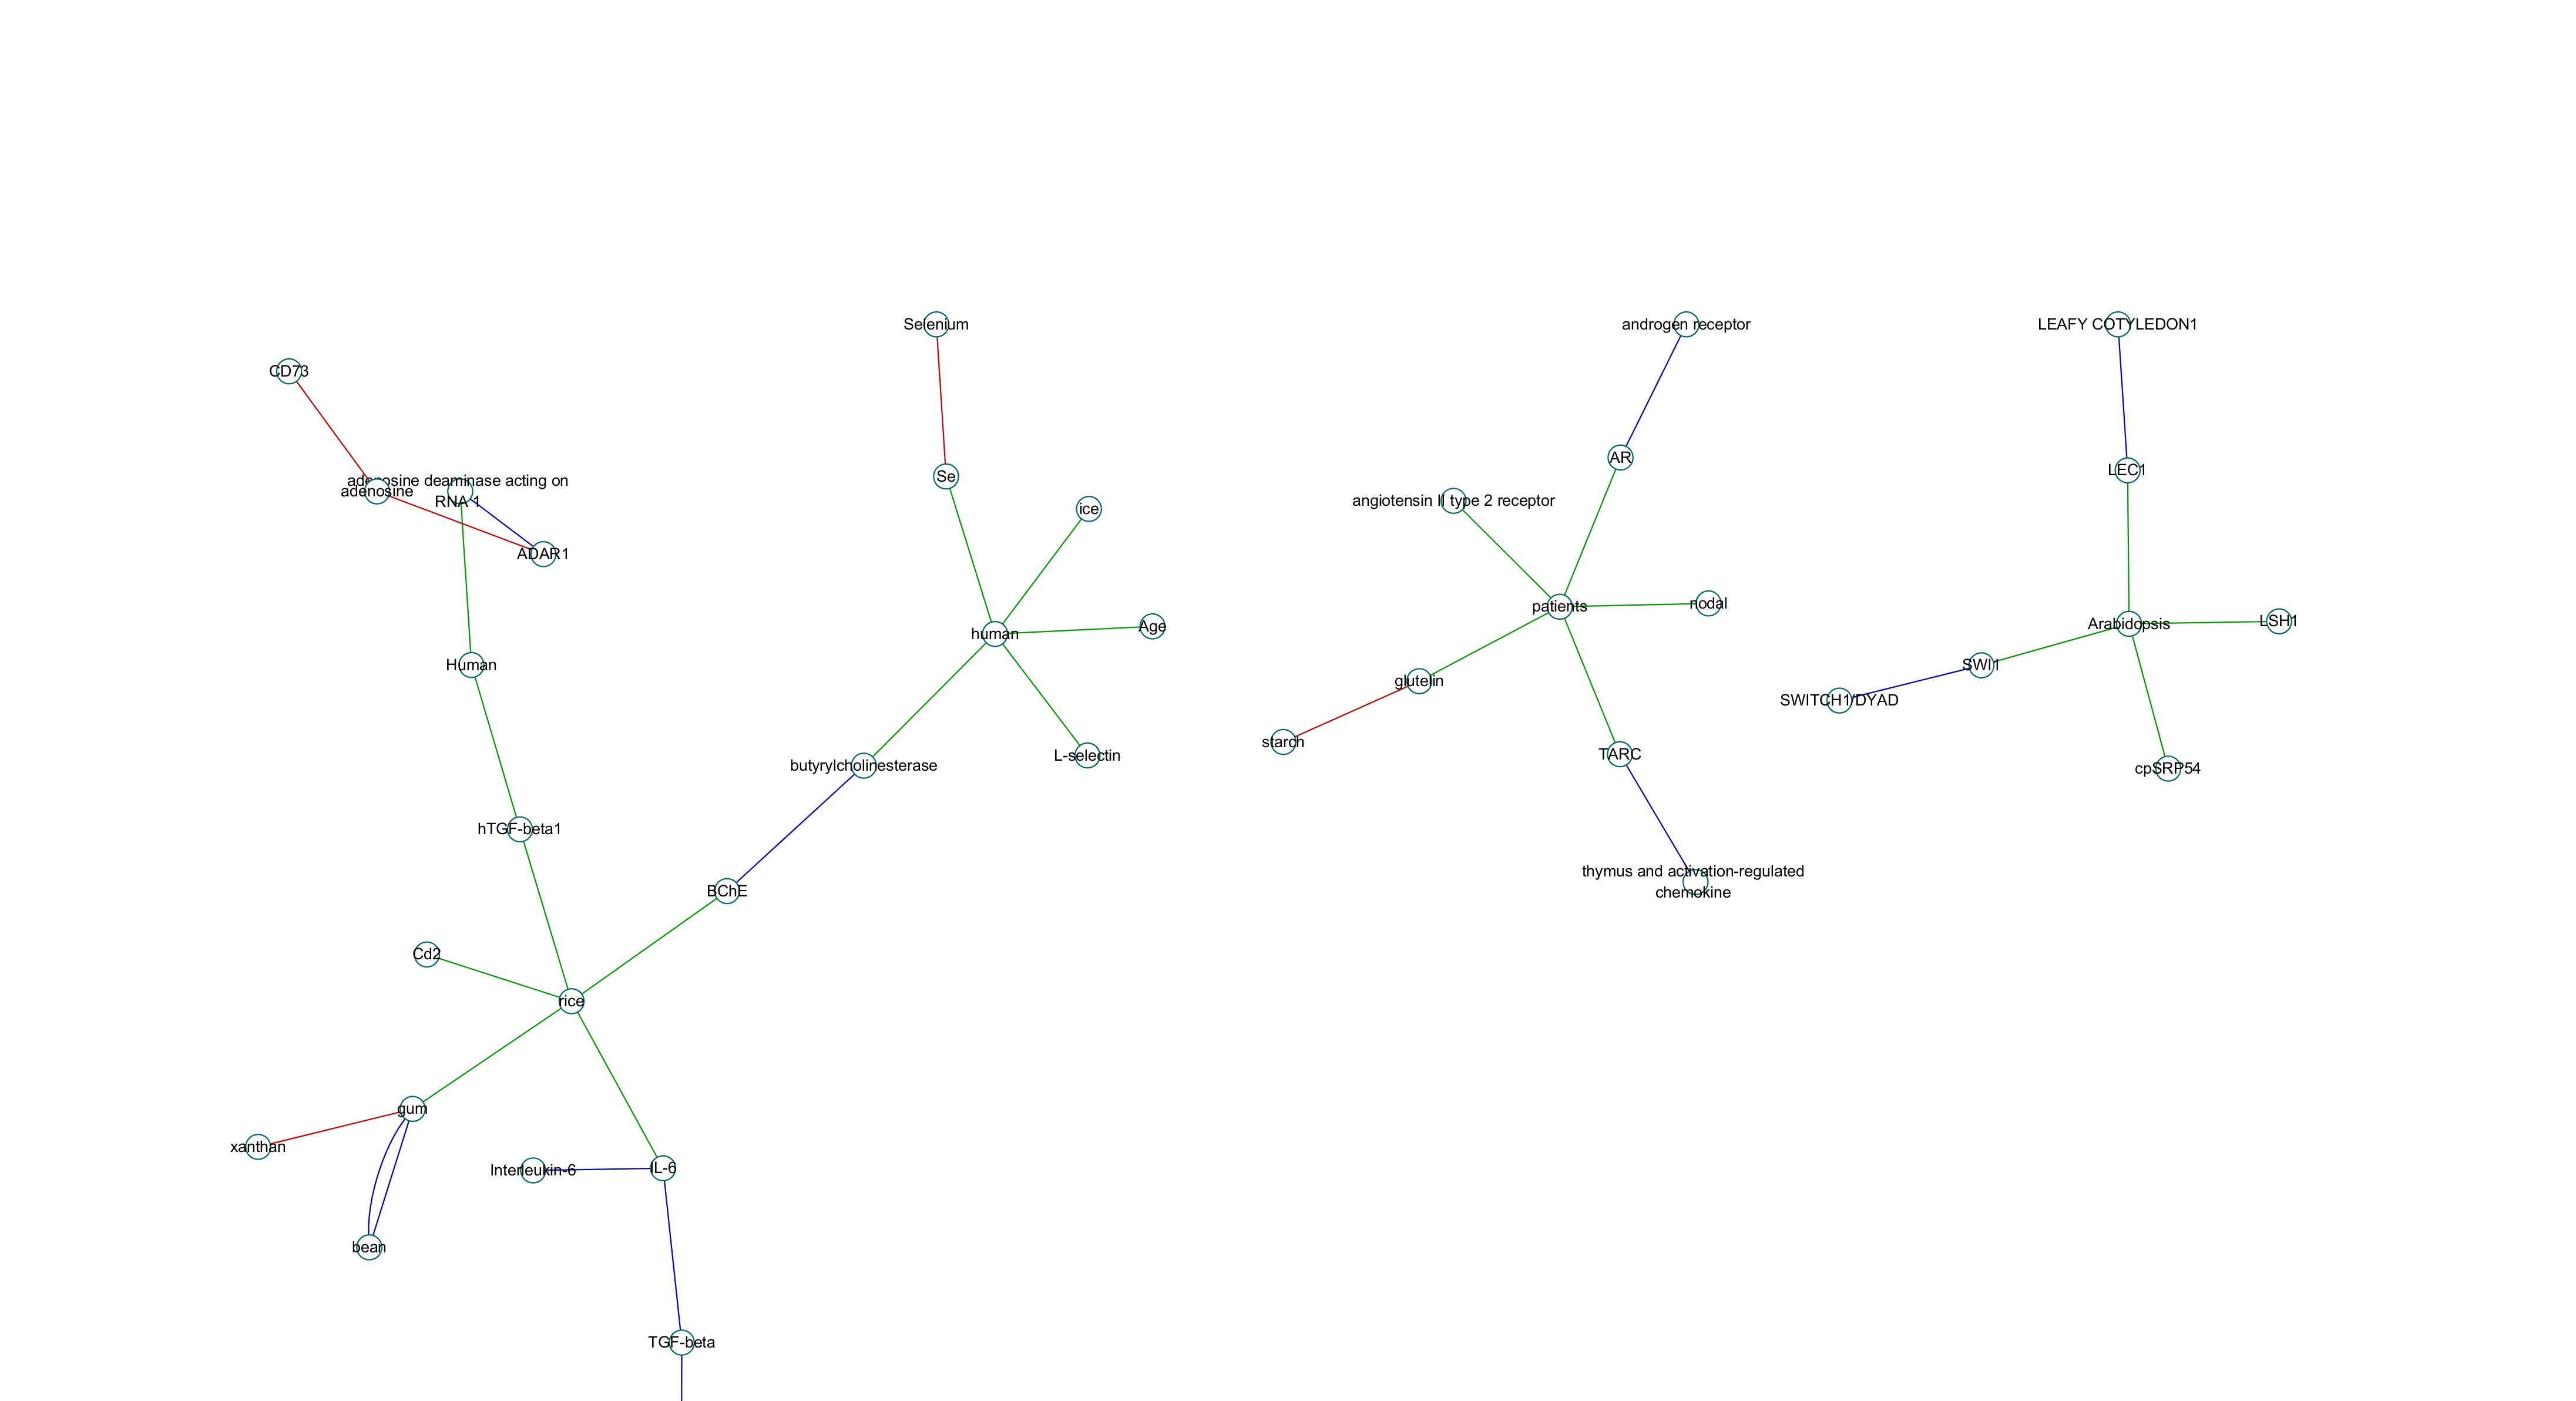
\includegraphics[scale=0.10]{./picture/Gene.png} %1.png是图片文件的相对路径
  \caption{Gene的相互作用网络局部图} %caption是图片的标题
  \label{mmmss} %此处的label相当于一个图片的专属标志,目的是方便上下文的引用
\end{figure}
居然在下方还可以看到挖出了新冠病毒和他的主要受体ACE2(见图\ref{gene2})。估计是搜索文献时混入了其他文献。并且这5,395篇文献的数目还是太少了,导致了整个网络不够大,不足以反映出更加好看的关联和解释性。网络下方还有很多单个单个的相互作用对,且以\textcolor{blue}{Gene-Gene}出现居多。


\begin{figure}[H]
  \centering
  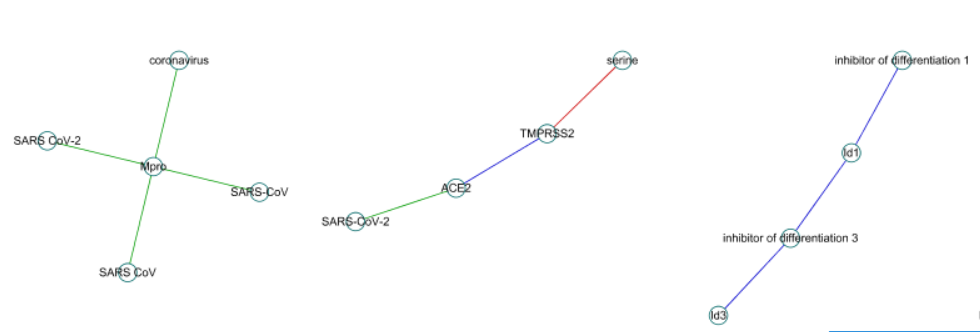
\includegraphics[scale=0.6]{./picture/Gene2.png} %1.png是图片文件的相对路径
  \caption{Gene的相互作用网络局部图2} %caption是图片的标题
  \label{gene2} %此处的label相当于一个图片的专属标志,目的是方便上下文的引用
\end{figure}
	\subsubsection{Chemical的相互作用网络局部图}
	设置Tools--Network Analyzer---Network Analysis----Generate Style from Statistics,我们可以更直观的分析Chemical为主的相互作用网络(见图\ref{sssddffgg})。设置的是度越大节点越大,可以从图中看节点越大的互作对象比较多。这里依旧是rice。同时用节点的颜色来表示接近中心性,也就是一个节点和其他节点沟通的最短路径的平均值,衡量传递速度。越红意味着它们想要沟通其他实体所需要跨过的人越多。边介度越大边越粗,边承载流量的能力越大,这些较粗的边上节点可以看作“核心节点”。
	这里的红色是\textcolor{red}{化学物质-物种},蓝色是\textcolor{blue}{化学物质-化学物质},绿色是\textcolor{green}{化学物质-基因}。
	\begin{figure}[H]
  \centering
  \includegraphics[scale=0.1]{./picture/Chemical.png} %1.png是图片文件的相对路径
  \caption{Chemical的相互作用网络局部图2} %caption是图片的标题
  \label{sssddffgg} %此处的label相当于一个图片的专属标志,目的是方便上下文的引用
\end{figure}
比如我们把目光放在核心节点“rice”上(见下图\ref{asjdiajhsd})。它像是一个“花蕊”,而周围辐射状的是花瓣。实际上是因为他和后写节点出现的次数非常多,有很多条连边导致的。我们用黄色选中了它本身和它的直接邻居。可以看到周围几乎都是“rice”的邻居。然后我们观察和它相互作用频次比较多的几个节点,可以看到相关的红色节点——也就是和水稻这个物种相关的化学物质主要有:water、carbon、nitrogen、salt、starch(淀粉)等。都是在水稻生长过程中比较重要也比较常见的化学物质。\par
然后蓝色的边,主要反应化学物质-化学物质之间的相互作用。可以观察到Cd和Cadium(镉)共现的频率比较高。还有N和nitrogen以及carbon、methane和CH4。也就是说,共现频率太高往往说明这两种名称指代的是相同的东西。
	\begin{figure}[H]
  \centering
  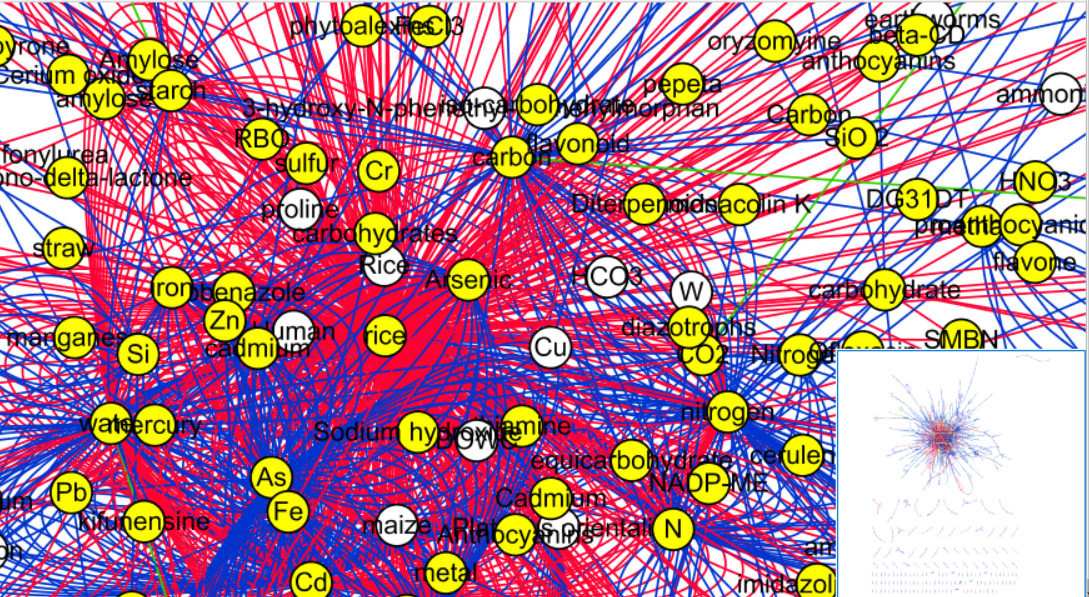
\includegraphics[scale=0.5]{./picture/rice.png} %1.png是图片文件的相对路径
  \caption{rice节点及其邻居} %caption是图片的标题
  \label{asjdiajhsd} %此处的label相当于一个图片的专属标志,目的是方便上下文的引用
\end{figure}

	\section{结论与展望}
	其实由于时间比较匆忙,整个过程有很多待完善的地方,细节上比较简单的比如可以将所有的词汇转化为小写这样就不会在图\ref{xxxxxxx}中既看见Rice也出现rice了。\par
	受限于篇幅和时间的原因,这里不再具体展开。总之本次实验虽然只是利用非常非常简单的代码,观察共句信息。但是依旧发现了一些知识。\par
	
	\section{Github链接}
	代码详见:\par
	\href{https://github.com/LianzePuppet/nlp.homework4}{\underline{Github链接}}:https://github.com/LianzePuppet/nlp.homework4

\section{参考链接}
\begin{enumerate}
\item \href{https://my.oschina.net/indexofire/blog/1492062}{\underline{玩转 edirect}}
\item \href{https://blog.csdn.net/u012390519/article/details/74231606}
{\underline{shell中的curl网络请求}}
\item \href{https://blog.csdn.net/zhanyongjia_cnu/article/details/50717717}
{\underline{Entrez Direct学习笔记}}
\item \href{https://mp.weixin.qq.com/s/bndecTSABox2dcr7aoheig}
{\underline{R包安利 ② pubmed.mineR—又一个PubMed利器}}
\item \href{https://zhuanlan.zhihu.com/p/220527695}
{\underline{一网打尽:cytoscape详细教程}}
\end{enumerate}
\bibliographystyle{unsrt}
\bibliography{MyCitation}% Produces the bibliography via BibTeX.
\end{document}


















%%%%%%%%%%%%%%%%%%%%%%%%%%%%Library%%%%%%%%%%%%%%%%%%%%%%%%%%%%%%%%%%%%%%%

% 1. 脚注用法
	LaTeX\footnote{Latex is Latex} is a good software

%2. 强调
	\emph{center of percussion} %[Brody 1986], %\lipsum[5]

%3. 随便生成一段话
	\lipsum[4]

%4. 列条目
	\begin{itemize}
	\item the angular velocity of the bat,
	\item the velocity of the ball, and
	\item the position of impact along the bat.
	\end{itemize}

%5. 表格用法
	\begin{table}[h]
	\centering  
	\begin{tabular}{c|cc}
		\hline
		年份 & \multicolumn{2}{c}{指标}\\
		\hline
		2017 & 0.9997 & 0.0555 \\
		2018 & 0.9994 & 0      \\
		2019 & 0.9993 & 0      \\
		\hline
	\end{tabular}
	\caption{NAME}\label{SIGN}
	\end{table}

	\begin{center}
		\begin{tabular}{c|cclcrcc}
			\hline
			Year & theta & $S_1^-$ & $S_2^-$ & $S_3^-$ & $S_4^+$ & $S_5^+$ & $S_6^+$ \\%表格标题
			\hline
			2016 & 1      & 0      & 0 & 0.0001 & 0      & 0      & 0 \\
			2017 & 0.9997 & 0.0555 & 0 & 0.2889 & 0.1844 & 0.463  & 0 \\
			2018 & 0.9994 & 0      & 0 & 0.0012 & 0.3269 & 0.7154 & 0 \\
			2019 & 0.9993 & 0      & 0 & 0      & 0.4325 & 1.0473 & 0 \\
			2020 & 0.9991 & 0      & 0 & 0      & 0.5046 & 1.2022 & 0 \\
			2021 & 0.999  & 0      & 0 & 0      & 0.5466 & 1.2827 & 0 \\
			2022 & 0.9989 & 0.0017 & 0 & 0.3159 & 0.562  & 1.2995 & 0 \\
			2023 & 0.9989 & 0      & 0 & 0.0109 & 0.5533 & 1.2616 & 0 \\
			2024 & 0.9989 & 0      & 0 & 0      & 0.5232 & 1.1769 & 0 \\
			2025 & 0.9989 & 0      & 0 & 0.1009 & 0.4738 & 1.0521 & 0 \\
			2026 & 0.9991 & 0      & 0 & 0      & 0.4071 & 0.8929 & 0 \\
			2027 & 0.9992 & 0.0004 & 0 & 0.1195 & 0.3248 & 0.7042 & 0 \\
			2028 & 0.9994 & 0.0164 & 0 & 0.046  & 0.2287 & 0.4902 & 0 \\
			2029 & 0.9997 & 0      & 0 & 0.0609 & 0.12   & 0.2545 & 0 \\
			2030 & 1      & 0      & 0 & 0      & 0      & 0      & 0 \\
			\hline
		\end{tabular}
	\end{center}

%6. 数学公式
	\begin{equation}
		a^2 = a * a\label{aa}
	\end{equation}
	
	\[
	\begin{pmatrix}{*{20}c}
	{a_{11} } & {a_{12} } & {a_{13} }  \\
	{a_{21} } & {a_{22} } & {a_{23} }  \\
	{a_{31} } & {a_{32} } & {a_{33} }  \\
	\end{pmatrix}
	= \frac{{Opposite}}{{Hypotenuse}}\cos ^{ - 1} \theta \arcsin \theta
	\]
	
	\[
	p_{j}=\begin{cases} 0,&\text{if $j$ is odd}\\
	r!\,(-1)^{j/2},&\text{if $j$ is even}
	\end{cases}
	\]
	
	
	\[
	\arcsin \theta  =
	\mathop{{\int\!\!\!\!\!\int\!\!\!\!\!\int}\mkern-31.2mu
		\bigodot}\limits_\varphi
	{\mathop {\lim }\limits_{x \to \infty } \frac{{n!}}{{r!\left( {n - r}
				\right)!}}} \eqno (1)
	\]

%7. 双图并行
	\begin{figure}[h]
		% 一个2*2图片的排列
		\begin{minipage}[h]{0.5\linewidth}
			\centering
			\includegraphics[width=0.8\textwidth]{./figures/0.jpg}
			\caption{Figure example 2}
		\end{minipage}
		\begin{minipage}[h]{0.5\linewidth}
			\centering
			\includegraphics[width=0.8\textwidth]{./figures/0.jpg}
			\caption{Figure example 3}
		\end{minipage}
	\end{figure}

%8. 单张图片部分
	\begin{figure}[h]
		%\small
		\centering
		\includegraphics[width=12cm]{./figures/mcmthesis-aaa.eps}
		\caption{Figure example 1} \label{fig:aa}
	\end{figure}

%%%%%%%%%%%%%%%%%%%%%%%%%%%%%%%%%%%%%%%%%%%%%%%%%%%%%%%%%%%%%%%%%%%%%%%%%%%%%
\begin{minipage}{0.5\linewidth}
	\begin{tabular}{|c|c|c|}
		\hline
		\multicolumn{2}{|c|}{\multirow{2}{*}{合并}}&测试\\
		\cline{3-3}
		\multicolumn{2}{|c|}{}& 0.9997  \\
		\hline
		2019 & 0.9993 & 0 \\
		\hline
	\end{tabular}
\end{minipage}

\begin{minipage}{0.5\linewidth}
	\begin{tabular}{c|ccc}
		\hline
		年份 & \multicolumn{3}{c}{指标}\\
		\hline
		\multirow{3}{*}{合并}&2017 & 0.9997 & 0.0555 \\
		&2018 & 0.9994 & 0      \\
		&2019 & 0.9993 & 0      \\
		\hline
	\end{tabular}
\end{minipage}



	\begin{table}[h]
	\centering	
	\begin{Large}
		\begin{tabular}{p{4cm} p{8cm} < {\centering}}
			\hline
			院\qquad 系: & 信息工程学院 \\
			\hline
			团队名称: & PlantBook Team \\
			\hline
			分\qquad 组: & 第0组1号 \\
			\hline
			日\qquad 期: & 2017年10月28日 \\
			\hline
			指导教师: & 吱吱吱\\
			\hline
		\end{tabular}
	\end{Large}
\end{table}


\ctexset{
	section={
		format+=\heiti \raggedright,
		name={,、},
		number=\chinese{section},
		beforeskip=1.0ex plus 0.2ex minus .2ex,
		afterskip=1.0ex plus 0.2ex minus .2ex,
		aftername=\hspace{0pt}
	},
}

	\begin{table}[h]
	\centering
	\begin{Large}
		\begin{tabular}{p{3cm} p{7cm}<{\centering}}
			院  \qquad  系: & 信息工程学院           \\ \cline{2-2}
		\end{tabular}
	\end{Large}		
\end{table}
\thispagestyle{empty}
\newpage
\thispagestyle{empty}
\tableofcontents
\thispagestyle{empty}
\newpage
\setcounter{page}{1}

% 9. 代码

\usepackage{listings}
\usepackage{xcolor}
\lstset{
	numbers=left, 
	numberstyle= \tiny, 
	keywordstyle= \color{ blue!70},
	commentstyle= \color{red!50!green!50!blue!50}, 
	frame=shadowbox, % 阴影效果
	rulesepcolor= \color{ red!20!green!20!blue!20} ,
	escapeinside=``, % 英文分号中可写入中文
	xleftmargin=2em,xrightmargin=2em, aboveskip=1em,
	basicstyle=\footnotesize,
	framexleftmargin=2em
}
